%% content.tex
%%
\chapter{Randomized Algorithms}
\label{ch:randomizedAlgorithms}

\section{Preamble}
The following Algorithms work using the $\mathcal{CONGEST}$ model. This means that we design the algorithm to function on our class of graphs described earlier when we analyzed what forms of graphs appear in the SINR model. We assume that in one broadcast round there is one message sent to all neighbors of a node and one received by each incoming edge for a node. The time to simulate a broadcast model in the $\mathcal{SINR}$ model is known to be $O(\Delta \log{n})$, with $\Delta$ being the maximum in-degree of all nodes and $n$ the number of nodes. This time is then re-substituted for a broadcast.
\todo{rework this and/or move it to preliminaries}

\section{Necessary Changes For Directed Graphs}
In the algorithms suggested Derbel and Talbi \cite{dt-dncsi-10} as well as in popular models like the $\mathcal{PROTOCOL}$ model, we assume to have uniform disk graphs. This assumption is a huge one to make, however, as the $\mathcal{SINR}$ model for example suggests a non-uniform disk graph, while the $\mathcal{DECAY}$ model goes even further and makes no assumptions about the structure of the graph anymore besides that its nodes have locations and cannot be arbitrarily moved in a graphical representation, creating a model closer to reality.

In this section, we will take the Algorithm 18, from Barenboim and Elkin \cite[p101]{be-dcg-13}, and make small changes to make it work in directed graphs.

We begin by introducing a helper function.


\begin{algorithm}[ht]
\DontPrintSemicolon 
\caption{\textsc{Get-K-Neighborhood(G)}}\label{alg:k-nghbr}
\SetKwFor{ForAll}{for}{do}

$N^0_v \defines (v, \emptyset)$\;

\ForAll{$i = 1 \dots K$}
{

\SetKwFor{ForEach}{for each}{do}

	send $N^{i-1}_v$\;

	$T = \emptyset$ \;

\ForEach{$N^{i-1}_u$ received}
{

$T = T \cup \{N^{i-1}_u\}$\;

$N^{i}_v \defines (v, T)$\;


}


}

return $N^k_v$

\end{algorithm}

\todo{describe this algorithm further}

This algorithm makes the $K$-neighborhood of a node known to that node. Its runtime depends on how many hops worth of neighborhood one needs to discover, which is represented by the parameter $K$. The procedure takes $O(\Delta^{K-1})$ rounds to complete, as for a 1-Neighborhood, a simple communication round suffices, a 2-Neighborhood requires every node to send and receive the data about its $\Delta$ neighbors, for a 3-Neighborhood, a node has to send $\Delta$-messages for each of its $\Delta$ neighbors, resulting in $\Delta^2$ messages, and so on.

Let us now go ahead and modify the algorithm.
\begin{algorithm}[ht]
\DontPrintSemicolon 
\caption{\textsc{Rand-2-Delta}}\label{alg:r2d}

Run Get-$2$-Neighborhood \;
Let $D_v$ be the set of nodes that dominate $v$, calculated from $v$'s 2-neighborhood\;

Let $T_v = \emptyset$, the set of temporary colors of the neighbors of $v$\;
Let $F_v = \emptyset$, the set of final colors of the neighbors of $v$\;
Let $N_v = \emptyset$, the set of neighbors of $v$ which have terminated\;

\SetKwFor{ForEach}{for each}{do}

\ForEach{round}{
	$T_v = \emptyset$\;
	$c_v :=$ draw a color from $[2\Delta]$ randomly\;
	send the color $c_v$ to all neighbors\;
	\ForEach{received color $c_u$ from a neighbor $u$}{
		$T_v = T_v \cup \{c_u\}$\;
	}\;
	\label{line:condition}\If{$c_v \notin T_v \cup F_v$ and $D_v \subseteq N_v$}{
		send the message "final $c_v$" to all neighbors\;
		select $c_v$ as the final color of $v$ and terminate\;
	}
	\Else{
		\ForEach{received message "final $c_u$" from a neighbor $u$}{
			$F_v = F_v \cup \{c_u\}$\;
			$N_v = N_v \cup \{u\}$\;
		}
		discard $c_v$ and continue to the next round
	}
}

\end{algorithm}

At first we detect the local neighborhood of a node $v$ by broadcasting its identity, and then broadcasting all identities that $v$ has received. That way we know which nodes we can receive but not send to, which we save to $D_v$. Until all nodes in $D_v$ have terminated, $v$ only superficially joins the rounds of picking colors, as it never terminates before then. In each round, $v$ picks a random color from the pool $[2\Delta]$ and broadcasts it. If no neighbor picked the same color in the round or terminated with that color previously, and if $D_v$ is terminated, $v$ sends out the chosen color as "final $c_v$" and stops.

\begin{lemma}
\label{theorem:r2dproof}
  Algorithm Rand-2Delta produces a legal $2\Delta$-vertex-coloring when all nodes terminate
\end{lemma}
\begin{proof}
  Let us choose a pair of neighbors arbitrarily, $u,v \in V$. Let $i,j$ be the rounds in which these nodes terminate respectively.
	
	\textbf{case } $i < j$: \\
	We also look at $j < i$ in this case by simply switching the roles of $u$ and $v$.\\
	For contradiction we assume that final $c_v = $ final $c_u$ and look at additional cases:
	
	
	\hspace{10pt}\textbf{case } $u$ dominates $v$: \\
	In the case that $v$ is dominated, it only chooses a final color when $u$ has chosen its final color, and $v$ cannot end with the same color (Line \ref{line:condition}).
	
	\hspace{10pt}\textbf{case } $v$ dominates $u$: \\
	Directly contradicts $i < j$, as $v$ will terminate before $u$ (Line \ref{line:condition}).
	
	
	\hspace{10pt}\textbf{case } $v$ and $u$ communicate: \\
	As $u$ terminates before $v$ does, $v$ knows "final $c_u$" is taken and cannot terminate using that (Line \ref{line:condition}) .
	
	\textbf{case } $i = j$: \\
	In this case, both nodes terminate at the same time. As Line \ref{line:condition} requires that no neighbor of a node has the same color for the node to terminate (either temporary or finalized), $c_u \neq c_v$ and both nodes terminate with different colors.
\end{proof}

\begin{lemma}
\label{theorem:r2dzeit}
	Let $G_1$ be the subgraph of G, that contains all nodes that are not dominated by another node. Formally, $G_1 := (V_1 := \{v \in V : D_v = \emptyset \}, E)$. Algorithm \ref{alg:r2d} will produce a valid coloring for $G_1$ in $O(\log n)$ rounds, with a probability over $1-1/n^c$ for an arbitrarily large constant $c$.
\end{lemma}
\begin{proof}
	Similarly to Barenboim and Elkin \cite[p. 102]{be-dcg-13}, we argue that for a given node $v \in V_0$, the probability that it has chosen a color of one of its neighbors is at most $\Delta / 2\Delta$, the maximum number of neighbors divided by the size of the pool to choose its color from.
	
	Consequently, the probability that $v$ has not finished in round $i$ is $(1/2)^i$. By the union bound, the probability that such a $v$ exists for a given round $i$ is at most $n \cdot (1/2)^i$. (We could argue that instead of $n$, the number of nodes in the subgraph, $m = |V_1|$ suffices here. \todo{is this true?} However, as $m \leq n$, we will be using $n$ hereafter to simplify the proof.)  Hence, after $(c+1) \cdot \log n$ rounds, with probability not less than $1-n \cdot (1/2)^i \geq 1-1/n^c$, all of these nodes terminate successfully.
\end{proof}

Let us now define a family of subgraphs recursively, starting with $G_1$, which had been defined earlier. We define $G_{k+1}$ as the subgraph, that includes all nodes which are dominated only by nodes of $G_k$, formally: $G_{k+1} \defines (V_{k+1} \defines \{v \in V : D_v \subseteq V_k\}, E)$. This family holds an invariant: $V_k \subseteq V_{k+1}$.

\begin{lemma}
\label{theorem:r2dlaenge}
	$\exists N \in  \mathbb{N} : \forall k \geq N : G_k = G$
\end{lemma}
\begin{proof}
	Let us choose $k$ so that $G_k = G_{k+1}$, it is sufficient to show that in that case $G_k = G$ already.
	Assume for contradiction that $G_k \neq G$. This means that in round $k+1$, no new nodes get added to the subgraph, so $V_k = V_{k+1} \neq V$. 
	
	We define $C \defines V \backslash V_k$ as the set of nodes which are not being added to the subgraph family, $C \neq \emptyset$. For an arbitrary node $v \in C$ this means that $D_v \cap C \neq \emptyset$, as $D_v$ contains at least one node $u$ that isn't in $V_k$.
	
	This implies that $|C| \geq 3$, since two nodes cannot dominate each other (that would be simply bidirectional communication). As for a given node $v$, we always have a node $u \in C$ which dominates it and therefore we can hop indefinitely to the next dominator. As we can do over $|C|$ hops, this implies that $C$ contains a cycle.
	
	This contradicts the definition of our graphs, namely that they cannot have strictly directed cycles.
\end{proof}
Further on, we define $l$ as the smallest such $N$. $l-1$ is the length of the longest, strictly directed path in $G$. We will see later on that the algorithm works even without the constraint of having no cycles, obviously we cannot have an $l$, then, though, as the length of the longest, strictly directed path in that case is infinite. \todo{reference the min(l, log n) here}

\begin{lemma}
\label{theorem:r2diteration}
	For a legally colored $G_k$, Algorithm \ref{alg:r2d} needs, with probability not less than $1-1/n^c$ for an arbitrarily large constant c, $O(\log n)$ further rounds to legally color $G_{k+1}$
\end{lemma}
\begin{proof}
	If $G_k = G$ we're already done.
	So we assume $G_k \neq G$.\\
	We choose a node $v$ out of the set $V_{k+1}\backslash V_k$ arbitrarily. Similarly to the first iteration, we argue that the probability for $v$ to still conflict with other nodes, and so to not being finished in round $i$ is at most $(\Delta /(2\Delta))^i = (1/2)^i$. We turn that around and argue that the probability for such a $v$ to exist in round $i$ is at most $n (1/2)^i$, and again after $(c+1) \cdot \log n$ rounds, with probability not less than $1-n \cdot (1/2)^i \geq 1-1/n^c$, all of these nodes terminate successfully.
\end{proof}

\begin{theorem}
\label{theorem:r2dkomplett}
	We conclude that Algorithm \ref{alg:r2d} needs, with probability not less than $1-1/n^c$ for an arbitrarily large constant c, $O(\Delta + l \cdot \log n)$ rounds to terminate successfully.
\end{theorem}
\begin{proof}
	The sub-procedure Get-$2$-Neighborhood requires $O(\Delta)$ rounds to complete, as shown earlier. Combining the three previous theorems, we need $O(\log n)$ rounds to compute $G_1$, then we need $l$ times $O(\log n)$ rounds to for all nodes in $G_l = G$ to terminate, at which point all nodes are legally colored. \todo{combine the probabilities}
\end{proof}

\section{Simplifying the Algorithm}

In order to get rid of the $\Delta$-factor in Algorithm \ref{alg:r2d}, we will need, of course, to remove the neighborhood-search, and to make a few adjustments to the algorithm itself, as a node will never know if it is still dominated or not, it can never know whether it has terminated or is still running. For this, we will increase the amount of colors from $2\Delta$ to $3\Delta$.

\begin{algorithm}[ht]
\DontPrintSemicolon 
\caption{\textsc{Rand-3-Delta}}\label{alg:ir2d}

Let $T_v = \emptyset$, the set of colors of the neighbors of $v$\;

$c_v \defines$ draw a color from $[3\Delta]$ randomly\;

\SetKwFor{ForEach}{for each}{do}

\ForEach{round}{
	$T_v = \emptyset$\;
	send the color $c_v$ to all neighbors\;
	\ForEach{received color $c_u$ from a neighbor $u$}{
		$T_v = T_v \cup \{c_u\}$\;
	}\;
	

	\If{$c_v \in T_v$}
	{
		redraw $c_v$ from $[3\Delta] \backslash T_v$
		}\label{alg:ir2d:while}
}

\end{algorithm}

\todo{describe the algorithm}

This algorithm looks much simpler than Algorithm \ref{alg:r2d}, however the latter is easier to prove to be working correctly, and we will be using it as a stepping stone to prove the former.

Even though the nodes don't know the set of their dominating nodes $D_v$, for the proof we will still use this set as defined in Algorithm \ref{alg:r2d}. We will also use the family of subgraphs defined in \ref{theorem:r2dzeit}.

As nodes cannot enter the state \textit{terminated} anymore, because of their lack of knowing their dominating nodes, we will introduce the notion of a \textit{stable} node. A node is stable when it never changes its color in the future anymore. Obviously a node cannot know when it will be stable itself, either.

\begin{lemma}\label{lemma:ir2d-proof}
	When all nodes are stable, Algorithm \ref{alg:ir2d} produced a legal $3\Delta$ coloring of $G$.
\end{lemma}
\begin{proof}
	Let us assume for contradiction that for two neighboring nodes $u$ and $v$, $c_u = c_v$, then either one (in case one is dominated by the other) or both nodes redraw their colors and hence are not stable.
\end{proof}

\begin{lemma}\label{lemma:ir2d-redraw}
	A node $v$ is stable when $D_v$ is stable and $v$ has stopped redrawing once since then.
\end{lemma}
\begin{proof}
	If we assume that $v$ did not need to redraw in round $i$, but needs to redraw in round $i+1$, which means that some other node $u$ picked the color $c_u = c_v$, it follows that either $v$ was dominated by $u$, in which case $u \in D_v$ should have been stable already, or $u$ picked $c_u \notin T_u$ which contradicts line~\ref{alg:ir2d:while}, since $c_v \in T_u$.
\end{proof}

\begin{lemma}\label{lemma:ir2d-zeit}
	The subgraph $G_0$, with high probability, is stable after $O(\log n)$ rounds.
\end{lemma}
\begin{proof}
	For an arbitrary node $v \in V_1$, the chance that it conflicts in the first round is $\Delta / 3\Delta = 1/3 < 1/2$. For each successive round, the pool of colors $v$ can choose from is at least $2\Delta$ as at most $\Delta$ colors may be blocked. In the worst case, all neighbors switch to a new color and the chance that $v$ is in a conflict again is at most $\Delta / 2\Delta = 1/2$, the number of all neighbors choosing a new color divided by their pool.
	
	As we did for Algorithm \ref{alg:r2d}, using Lemma \ref{lemma:ir2d-redraw} (as $D_v = \emptyset$, which obviously is stable), we can now argue that the chance for a node to not be stable in round $i$ is at most $1/2^i$ and by the union bound assert that the chance for such a node to exist is at most $n \cdot 1/2^i$. Again, after $(c+1) \cdot \log n$ rounds, with probability not less than $1-n \cdot (1/2)^i \geq 1-1/n^c$, there is no more such node.
\end{proof}

\begin{theorem}\label{theorem:ir2d}
	Algorithm \ref{alg:ir2d} produces, with high probability, a valid $3\Delta$-coloring of $G$ in $O(l \log n)$ rounds.
\end{theorem}
\begin{proof}
	As we showed before, we assert that for each iteration of $G_{k+1}$, it takes, with high probability, not longer than $O(\log n)$ rounds, as all dominating nodes of $G_{k+1}$ in $G_k$ are stable, the remaining nodes respect their chosen color and have, in the worst case, still at most $\Delta$ neighbors picking a new color. With that, again, we have the probability of a node $v$ having to redraw in round $i$ at most $(1/2)^i$, and use the same argument as before, finding that it takes $O(\log n)$ rounds to make $G_{k+1}$ stable. So, from Lemma~\ref{theorem:r2dlaenge} we can state that after $l \cdot O( \log n)$ rounds $G_l = G$ is stable and from Lemma~\ref{lemma:ir2d-proof} that Algorithm~\ref{alg:ir2d} indeed produced a valid coloring.
\end{proof}


Let us now improve this algorithm so that it works with a desirable $\Delta+1$ amount of colors.

\begin{algorithm}[ht]
\DontPrintSemicolon 
\caption{\textsc{Rand-Delta-Plus1}}\label{alg:rd+1}

Let $T_v = \{0\}$, the set of colors of the neighbors of $v$\;
Let $c_v = 0$ be an invalid color\;

\SetKwFor{ForEach}{for each}{do}

\ForEach{round}{

	\If{$c_v \in T_v$}
	{
		draw $c_v$ from $\{0,1\}$\;
		\If{$c_v = 1$}
		{
			redraw $c_v$ from $[\Delta+1] \backslash T_v$
		}
		
	}
	
	$T_v = \{0\}$\;
	
	
	send the color $c_v$ to all neighbors\;
	\ForEach{received color $c_u$ from a neighbor $u$}{
		$T_v = T_v \cup \{c_u\}$\;
	}
	
	

}

\end{algorithm}

\todo{proof}


\section{A Lower Bound}

We will now introduce a lower bound to randomized algorithms solving directed graphs.

\begin{theorem}\label{theorem:lowerbound}
For a randomized algorithm which produces valid $O(\Delta)$ colorings on any directed graph with high probability, there exists a lower bound of $\Omega (\min\{l, \log n\})$ rounds to compute it.

\end{theorem}
\begin{proof}
Let us look at a special kind of graph, a chain of single nodes dominating the next one. We will be using $v_1, \dots v_{l+1}$ to refer to the nodes.

\begin{figure}[ht]
\center
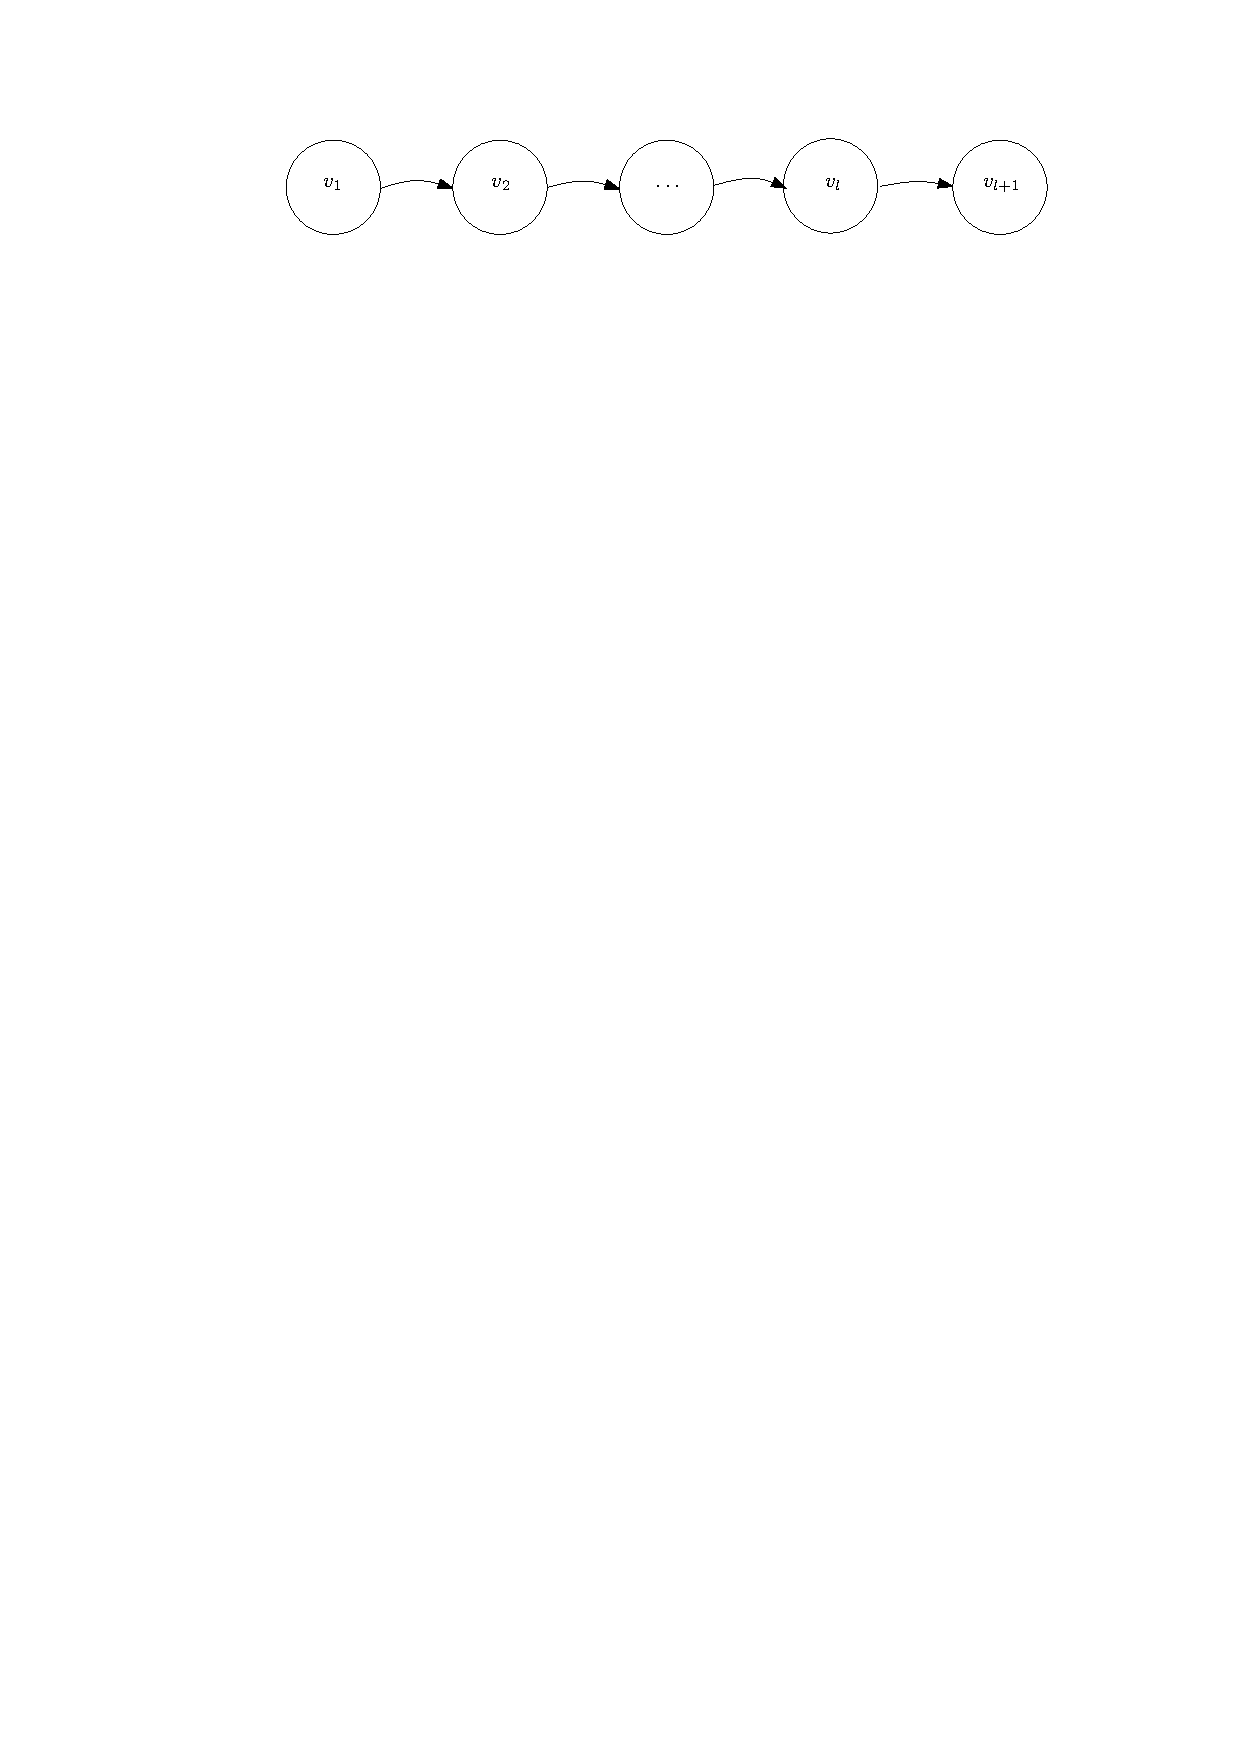
\includegraphics{figures/chain.pdf}
\caption{A graph consisting of a chain of dominating nodes}
\end{figure}

For each edge $(v_k, v_{k+1})$ there is a probability that it produces a conflict as one node is dominated and therefore cannot respect the choice of that color. There exists a constant $c>1$ so that this probability is greater or equal to $1/c$ for every edge.

Now, assuming in round $t$ there is a conflict, the probability for a conflict to happen in round $t+1$ is greater or equal to $1/c$, again. The probability of a conflict spreading $t$ rounds is greater or equals $1/c^t$.

For a round $t < \log n$ this means the probability of conflict spreading so far is 
\begin{align*}
\frac{1}{c^t} \geq \frac{1}{c^{\log n-1}} = \frac{c}{n} > \frac{1}{n} > \frac{1}{n^{\tilde{c}}} \text{ for a } \tilde{c} > 1.
\end{align*}
Turning this around, this means that the probability to have no more conflicts in round $t$ is lower than $1/n^{\tilde{c}}$ for an arbitrarily large $c\tilde{c} > 1$. This means that the algorithm cannot finish with high probability before $\log n$ rounds for this graph.

For any directed graph, we will simply look at the subgraph containing the longest such chain described earlier, the argument from before still applies, as long as $l$ is sufficiently large. If $l$ is smaller than $\log n$ however, then a conflict can be solved through bidirectional communication at the end of the chain and therefore doesn't have the probability greater or equal $1/c$ to conflict anymore.

This means that the lower bound is $l$ for small values, and $\log n$ for big values of $l$, or $\Omega (\min\{l, \log n\})$.
\end{proof}

We can now use Theorem~\ref{theorem:lowerbound} to show that strictly directed cycles still produce valid colorings.

\begin{lemma}
For the Algorithms \ref{alg:r2d}, \ref{alg:ir2d} and \ref{alg:rd+1}, we do not need to change anything to make them work with strictly directed cycles, but the parameter $l$ in their runtimes will get bigger.
\end{lemma}
\begin{proof}
We have argued before that if a strictly directed cycle exists, at some point a subgraph containing that cycle will not be added to the family of subgraphs $G_k$ anymore. Let $G_i$ be the biggest subgraph not containing the cycle and the nodes dominated by it, and let it be stable (or terminated). We will interpret the cycle as a path of infinite length.

After $(c+1) \cdot \log n$ rounds, with probability not less than $1 - 1/n^c$, no more conflicts are spreading through this cycle, using the same union bound as was used for conflicts in single nodes before, now we used it to bound the hops.

We add the cycle $C$ to the subgraph $G_{i+1}$ and continue to construct the subgraph family until $G_l = G$.
\end{proof}
\todo{ob das reicht??}




\section{Testzeug}

\begin{algorithm}[ht]
\caption{\textsc{Stateless-Rand-Delta1}}\label{alg:algsrd1}
\DontPrintSemicolon 

\SetKwData{C}{C}

\SetKwFor{ForAll}{forall}{do}

\SetFuncSty{textsc}

\SetKwFunction{randcolor}{random}
\SetKwFunction{sendcolor}{send}
\SetKwFunction{receiveColor}{receive}


\C 
$
\leftarrow 
\left\{ 
1, \dots , \Delta + 1 
\right\} 
$ 
\;


$c 
\leftarrow 
$
\C.\randcolor{} 
\;




\ForAll{timeslots}{ \sendcolor{$c$} \tcp{with a certain probability}
\If{$ w = $ \receiveColor{} }{
\C = \C$\backslash \{w\} $ \;
\If{$ c == w $}{
$ c =$ \C.\randcolor{} }
}

}



\end{algorithm}
